% document class settings
\documentclass[12pt, a4paper]{article}

% encoding
\usepackage[utf8]{inputenc}
\usepackage[T1]{fontenc}

% opmaak
\usepackage{microtype}
\usepackage{XCharter}
\usepackage[T1]{eulervm}
\usepackage[scale=0.9]{FiraMono}
\usepackage[margin=2.5cm]{geometry}

\usepackage{titlesec}

% code blocks
\usepackage{caption}
\usepackage[outputdir=build,newfloat]{minted}
\usemintedstyle{stata}
%\renewcommand\listingscaption{Example code}
\captionsetup[listing]{position=top, name=Example code}
\SetupFloatingEnvironment{listing}{name=Example code,listname=Example Code}
\setminted{
  autogobble=true,
  fontsize=\footnotesize,
  frame=lines,
  linenos=true,
  bgcolor=azure,
  breaklines,
  breaksymbolleft={},
  breakindent=5ex
}
\usepackage{xcolor}
\definecolor{azure}{rgb}{0.93, 0.96, 0.96}


% from https://tex.stackexchange.com/questions/83204/how-can-i-make-source-code-included-with-minted-copyable
\usepackage{accsupp}
\newcommand\emptyaccsupp[1]{\BeginAccSupp{ActualText={}}#1\EndAccSupp{}}
\let\theHFancyVerbLine\theFancyVerbLine
\def\theFancyVerbLine{\rmfamily\tiny\emptyaccsupp{\arabic{FancyVerbLine}}}

\newcommand{\inputst}[1]{\inputminted{stata}{./Example do-files/#1}}
\newcommand{\st}[1]{\mintinline{stata}{#1}}%


%figures
\usepackage{graphicx}
\graphicspath{ {./figures} }

% regelafstand
\usepackage{setspace}
\onehalfspacing%

% header & footer
\usepackage{fancyhdr}
\pagestyle{fancy}
\fancyhead[L]{\small\itshape~Introduction to Stata Programming}%
\fancyhead[R]{\small\itshape\leftmark~}%
\fancyfoot[C]{\thepage}%
\setlength{\headheight}{14pt}%
\renewcommand{\sectionmark}[1]{%
  \markboth{#1}{}}%

% footnote spacing
\makeatletter%
\long\def\@makefntext#1{%
  \parindent 1em\noindent \hb@xt@ 1.8em{\hss \@makefnmark}\hskip2mm\relax#1}%
\makeatother

% bibliography
\usepackage[style=apa,natbib]{biblatex}
\addbibresource{references.bib}


% hyperlinks
\usepackage{hyperref}
\hypersetup{
  colorlinks=true,
  allcolors=black,
  linkcolor=blue,
  urlcolor=blue,
  citecolor=blue,
  linktocpage=true,
  hypertexnames=false
}
% pdf settings
\hypersetup{
    pdftitle=Introduction to Stata Programming,
    pdfauthor=Armin Hoendervangers,
    pdfdisplaydoctitle=true
}

% easy references to tables/figures etc
\usepackage[capitalise,noabbrev]{cleveref}
\crefname{listing}{Example code}{Example code}

% less "hanging" text at bottom or top of pages
\widowpenalty=10000
\clubpenalty=10000


\begin{document}

\begin{titlepage}\thispagestyle{empty}
    \begin{center}
        \vspace*{0.5cm}
        \LARGE
        Introduction to Stata Programming\\
        \Large
        Erasmus Thesis Project\\
        \vspace{1cm}
        \large
        Armin Hoendervangers\\
        AEclipse ETP Committee\\

        \vspace{2cm}
        Current version: \today\footnote{This is a work in progress, so the document will have incomplete sections and may contain mistakes.}

        \href{https://github.com/Ahvns/ETPreader/raw/main/Introduction%20to%20Stata%20Programming.pdf}{Click here for latest version}

        \vfill
    \end{center}
\end{titlepage}


\tableofcontents
\markboth{Contents}{}

\newcommand{\sectionbreak}{%
  \par%
  \begin{center}---\texttt{*}---\end{center}%
  \clearpage%
}%
\listoflistings


\section{Introduction}

Reader with advanced tips and tricks for Stata.
I'll add some introductory text about the reader here.
Incomplete sections will have a very short description of what will be described in them.
Could include some information about the thesis project, AEclipse, and maybe myself.
I assume some knowledge of and/or experience with both Stata and programming in general.
Comments and feedback are always welcome.


\section{Information Management}


Information is incredibly important in programming,
whether it is what a command does, how its used,
or what is contained in variables.
I take information as a starting point,
and this section is all about obtaining and storing various forms of information.


\subsection{The \texttt{help} command}

Perhaps the most important command in Stata,
\texttt{help} allows quick access to information on \emph{any} command Stata has.
The help-files Stata provides are incredibly detailed,
including information on how to use the command (its \emph{syntax}),
what the command does, its output, examples,
and sometimes even the theory behind it.
As useful as it is, the help-files might seem daunting at first.
Understanding their structure is key to (quickly) obtain information without falling into despair.
I'll highlight what I believe to be the most important parts of the help-files through an example.

If I type \mintinline{stata}{help summarize},
Stata opens the window in \cref{fig:hlpsum}.
In help-files, the typography on its own already gives us a lot of information.

\textbf{Bold} words indicate commands or options; if we want to use these,
we type them exactly as they are written down.
In our case,
\textbf{\texttt{summarize}} is written in bold under the syntax heading.
It is, as we know, indeed a command.

\textit{Italicised} text indicates something that should be substituted.
Here, \textit{\texttt{varlist}} tells us that we should write down a list of variable names here -- should we want to use this option.

Optional arguments and functions are indicated by being [in brackets].
This means that anything that is written within brackets in the syntax is something that does not have to be specified for a command to work.

\underline{Underlined} text indicates the \emph{minimum} abbreviation of a command or option.
In the case of \mintinline{stata}{summarize},
I could simply write \mintinline{stata}{su}.
Additional letters are also allowed and how to use this is mostly personal preference.
Personally, I always write \mintinline{stata}{sum} as its clearer to me what that means than \mintinline{stata}{su} would,
but it still saves me the time and space from writing the command out in its entirety.
When abbreviating commands,
make sure you are familiar enough with them to remember what an abbreviation means if you open your do-files one week later.
Having to look it up every time you see an abbreviation can be quite a pain.

Finally, any text in blue is a hyperlink,
generally leading to more information on whatever is written down.\footnote{~Note that the exact colour depends on Stata's colour scheme, but the default and dark schemes do use blue.}

\begin{figure}[tbp]\centering
  \caption{Help-file for \texttt{summarize}}\label{fig:hlpsum}
  \vspace{1ex}
  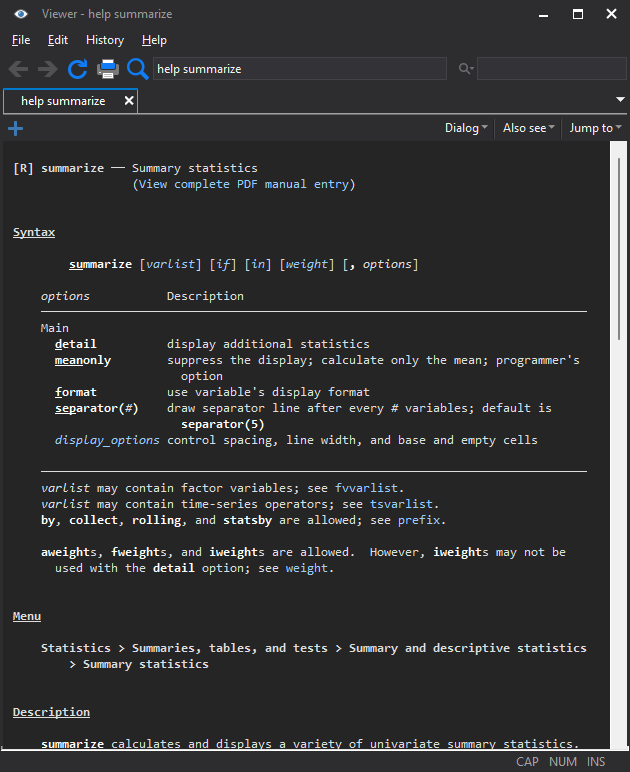
\includegraphics[width=0.85\textwidth]{helpsummarize}
\end{figure}

\subsection{scalars and matrices}

storing information in scalars and matrices

\subsection{display}

display command

\subsection{macros}

globals and locals


\section{Automation}


In this section we'll go over several commands that can be very useful for automating certain bits of code.

\subsection{Grouped command execution}
One of the easiest ways we can repeat a certain command for different groups of observations is with the \st{bysort} prefix.
This prefix lets us run the command we use it with for every group defined by a variable separately.
In my experience it's mostly useful for generating variables in programming,
but it can also be used as a quick and dirty way to compare variables across groups.
We can use the prefix like so: \st{bysort varlist: command},
where \st{varlist} is a list of the variables -- or a single variable --identifying the different groups,
and \st{command} is the command we would like to run.
Note that \st{bysort varlist:} is equivalent to using \st{by varlist, sort:}.
The \st{by} prefix does not work without sorting the data, so it is generally easier to just use \st{bysort}.
\cref{lst:sort} provides an example.

\begin{listing}[htp]
\caption{bysort.do}\label{lst:sort}
\inputst{bysort.do}
\end{listing}

\subsection{Conditionals}


\subsection{loops}

different types of loops


\section{Custom Commands}


Section on how to write a custom command.

\subsection{program}

defining a program

\subsection{arguments}

adding user input to a program

\subsection{syntax}

adding standard Stata syntax to a program

\subsection{temporary variables}

using temporary variables

\subsection{output}

defining program output


\section{General Tips}

Things I found helpful in using Stata.

\subsection{Coding stuff}

different types of comments

linebreaking commands

viewing multiple do-files side to side

do-file editor settings

\subsection{Customising Stata}

changing the font

changing Stata's colour scheme

\subsection{Project management}

folder structure

best practice for naming

multiple do-files

\subsection{Making nice output}

graphs

tables


%\printbibliography

\end{document}
